\documentclass{beamer}

\usepackage{../Research}

\newcommand{\F}{\mathcal F}
\newcommand{\curly}[1]{\left\{ #1 \right\}}


\title{A Tiny Example}
\author{Andrew Mertz and William Slough}
\date{June 15, 2005}


\begin{document}

\maketitle

\begin{frame}
	Suppose we have an (infinite) collection of sets $\F$. \\
	We define a shatter function $\pi_\F(n)$

	\begin{align*}
		\pi_\F(n) = \max \{ &\text {\# of atoms in boolean algebra generated by $S$} \\
		            &\mid S \subset \F \text{ with } |S| = n\}
	\end{align*}
\end{frame}

\begin{frame}
	Example: Let $\F$ consist of all discs on a plane.
	\begin{figure}[p]
    \centering
    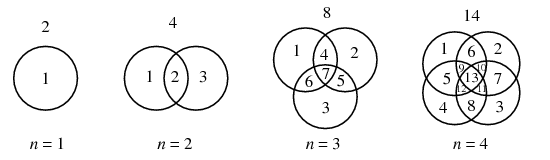
\includegraphics[scale=0.75]{circle.png}
	\end{figure}
	\begin{align*}
		\pi_\F(1) = 2 \ \ \  \pi_\F(2) = 4 \ \ \  \pi_\F(3) = 8  \ \ \ \pi_\F(4) = 14
	\end{align*}
	\begin{align*}
		\pi_\F(n) = \frac{1}{2}n^2 + \frac{1}{2}n + 1
	\end{align*}
\end{frame}

\begin{frame}
More examples: \\
	\begin{enumerate}
		\item Let $\F$ be a set of lines on a plane. Then
		\begin{align*}
			\pi_\F(n) &= n(n+1)/2 + 1
		\end{align*}
		\item Let $\F$ be a set of disks on a plane. Then
		\begin{align*}
			\pi_\F(n) &= n^2 - n + 2
		\end{align*}
		\item Let $\F$ be a set of balls in $\R^3$. Then
		\begin{align*}
			\pi_\F(n) &= n(n^2 - 3n + 8)/3
		\end{align*}
		\item Let $\F$ be a set of intervals on a line. Then
		\begin{align*}
			\pi_\F(n) &= 2n
		\end{align*}
		\item Let $\F$ be a set of half-planes. Then
		\begin{align*}
			\pi_\F(n) &= n(n+1)/2 + 1
		\end{align*}
		\item Let $\F$ be a collection of finite subsets of $\N$. Then
		\begin{align*}
			\pi_\F(n) &= 2^n
		\end{align*}
		\item Let $\F$ be a collection of polygons in a plane. Then
		\begin{align*}
			\pi_\F(n) &= 2^n
		\end{align*}
	\end{enumerate}
\end{frame}

\end{document}